\subsection{Challenges}
\label{sec:challenges}
\xiangyu{This section is updated.}
Achieving programmable resource management on GPUs remains fundamentally difficult today. 
Unlike CPUs—where extension frameworks such as eBPF provide stable, safe, and well-defined programmability points—GPU software stacks were not designed with similar goals. 
We identify three core challenges that make GPU programmability hard.

\subsection{C1: Lack of Safe and Stable Extension Points in Monolithic GPU Drivers}
Modern GPU drivers are large, monolithic vendor-controlled codebases that tightly intertwine low-level hardware mechanisms with proprietary resource-management policies, offering no stable hooks for user-defined logic. 
GPU drivers were not architected with programmable resource management in mind—partly due to historical assumptions about GPU usage, and partly due to strict safety constraints, as incorrect driver logic can stall the device or crash an entire node. 
As a result, developers cannot inject new scheduling policies, memory-placement strategies, or custom instrumentation without invasive modifications to vendor drivers. This absence of safe, stable extension points naturally limits any attempt to retrofit programmability into today's GPU stacks.

\subsection{C2: Mismatch Between CPU Extension Semantics and the SIMT GPU Execution Model}

\yusheng{mismatch between verify extension single thread CPU model vs SIMT GPU model, kernel concurrency / extension, not eBPF Semantics}

Even if GPU drivers exposed extensible interfaces, directly applying existing programmable CPU-oriented eBPF mechanisms does not work because of the conflict between eBPF semantics and the GPU Single Instruction Multiple Threads (SIMT) execution model execution model. 
Concretely, eBPF programs assume single-threaded control flow, strong memory consistency, and bounded execution enforced by a CPU-oriented verifier, whereas GPU kernels execute in warps of 32 threads that must follow largely uniform control paths. 
Naively running scalar eBPF logic per thread introduces warp divergence, unbounded serialization, and correctness risks stemming from thousands of simultaneous memory operations that the CPU-side verifier do not check. 
Furthermore, GPUs lack isolation, recovery points, or preemption mechanisms for misbehaving device-side code, meaning an unbounded loop or invalid access in policy logic can halt an entire device. 
The architectural and semantic mismatch makes straightforward reuse of eBPF unsafe and inevitably slow.

\subsection{C3: Absence of Efficient Mechanisms for Host–Device Shared State Status}

Even with GPU-side programmability that respects SIMT constraints, real GPU clusters require coordinated host–device resource management, which today lacks an efficient abstraction for shared policy state. 
GPU-accessible host memory suffers from orders-of-magnitude higher latency than GPU global memory, while GPU memory is capacity-limited and optimized for throughput, creating a fundamental mismatch in memory hierarchies. 
Meanwhile, CPU and GPU components operate asynchronously on vastly different timescales, causing policy decisions to rely on inconsistent state unless carefully synchronized. 
Existing systems force developers to manually manage DMA transfers, data replication, and consistency across devices, resulting in brittle, application-specific mechanisms that do not generalize.
The absence of a principled, efficient way to maintain shared state across the host–device boundary remains a major barrier to deploying practical programmable resource management on GPU clusters.

% Extending eBPF programmability to GPUs introduces fundamental challenges arising from (1) monolithic GPU drivers lacking designed-for-programmability interfaces, (2) fundamental mismatches between scalar eBPF semantics and GPU's SIMT execution model, and (3) complexities in coordinating consistent state across asynchronous host-device boundaries.
% \xiangyu{There is a mismatch between the description in this paragraph and the titles of 3.1-3.3.}
% \yusheng{we also need to change the title here to state the problems instead of goals?}

% \subsection{C1: Safe and Efficient Driver Extensibility}

% GPU drivers, such as NVIDIA's open GPU kernel modules, are large, monolithic codebases tightly integrating low-level hardware mechanisms and resource-management policies. While they expose APIs for applications to provide hints (e.g., \texttt{cudaMemAdvise}) or adjust parameters, these interfaces only allow applications to influence fixed built-in policies; they do not support defining custom algorithms such as FIFO eviction or tenant-aware scheduling. Unlike Linux kernel subsystems explicitly designed with stable eBPF extension points (e.g., \texttt{struct\_ops}), GPU drivers lack interfaces designed for policy programmability. \textbf{Policy logic embedded in driver mechanisms} complicates the introduction of attach points that remain stable across driver versions and GPU generations. For instance, in NVIDIA's Unified Virtual Memory (UVM) kernel module, the page-fault handler directly embeds LRU-based eviction and tree-based prefetch policies, making it difficult to interpose on memory placement without modifying the driver code path. Moreover, since policy logic executes directly in privileged driver contexts with tight latency constraints and direct GPU hardware control, there are \textbf{strict driver safety requirements}: logic errors (e.g., incorrect lock usage or inconsistent command submission) can cause device-wide stalls or node-level failures, mandating bounded execution and memory safety guarantees.

% \subsection{C2: SIMT-Aware Device-Side Execution}

% Standard eBPF is designed for scalar, single-threaded execution on CPUs, but GPU kernels operate under the fundamentally different Single Instruction Multiple Threads (SIMT) execution model, creating significant programmability mismatches. Naively mapping scalar eBPF handlers onto GPU threads introduces severe \textbf{warp divergence overhead}: executing scalar policy logic independently on all 32 threads of a warp forces the warp to serialize branches that depend on lane-local state, effectively turning each divergent branch into up to 32 serialized paths in the worst case. Furthermore, GPU architectures feature \textbf{memory bandwidth limit and complex synchronicity} and weak memory consistency semantics. For example, concurrent updates to shared maps from thousands of threads with relaxed atomics cannot be verified by the standard CPU-side eBPF verifier, which treats programs as single-threaded and cannot reason about SIMT interference. Lastly, GPU kernels execute within flat address spaces \textbf{without isolation or runtime recovery mechanisms}; policy errors like infinite loops or invalid memory accesses cause unrecoverable hardware stalls, making bounded execution and memory safety guarantees essential to enforce statically at compile time.

% \subsection{C3: Shared Cross-Layer State and Coordination}

% Many GPU policies require coordinated actions spanning CPU host drivers and GPU device execution; for example, GPU-side instrumentation capturing warp-level memory accesses informs host-side memory placement and scheduling decisions. Ensuring efficient and consistent cross-layer coordination poses unique technical difficulties. First, there is a significant \textbf{cross-boundary memory hierarchy mismatch}: placing shared maps naively in host memory introduces prohibitive latency (tens to hundreds of microseconds per access from GPU warps via PCIe), drastically impacting GPU utilization, whereas placing all shared state within GPU global memory or wrap local memory risks limited capacity, bandwidth bottlenecks, and cache thrashing. Second, host driver operations and GPU execution proceed asynchronously at vastly different granularities, complicating \textbf{state consistency}. High-latency propagation of GPU signals to host policies means that without careful coordination, host-side policy decisions (e.g., page eviction or kernel scheduling) risk relying on stale GPU-side signals (e.g., warp-level schedule statistics), causing thrashing migrations and oscillatory scheduling.

\section{\sys Design}

\subsection{Design Principles}

\sys follows three fundamental design principles:

% Any problem in computer systems can be sovled with another layer of indirection
\paragraph{Principle 1: Programmable Operating System Interface for GPU (os level?)  Programmability through (design Transparent and Dynamic Policy? Driver and DBI).}
\sys explicitly separates stable, privileged GPU driver mechanisms from dynamically programmable policies. Instead of embedding policies in opaque vendor stacks or application-specific runtimes, \sys provides clearly-defined policy interfaces that allow dynamic updates without requiring driver modifications or invasive application changes.

% A single model for exection and programming
% -> 
\paragraph{Principle 2: A single execution and programming model across the host and GPU.}
%execution and programming (a single Policy State and Control Plane)}
To eliminate the complexity and fragmentation of heterogeneous GPU stacks, \sys offers a unified abstraction for policy state, programming interfaces, and lifecycle management across CPU hosts and GPU devices. This ensures consistent cross-layer coordination, simplifies policy expression, and enables coherent decisions in asynchronous execution environments.

% compile time verifiation and optimization
\paragraph{Principle 3: Verifiable, SIMT-aware Safe and Efficient Execution.}
Recognizing the fundamental mismatch between traditional scalar eBPF semantics and GPU's SIMT parallelism, \sys introduces a static verification model explicitly designed for SIMT execution. Through a type discipline that distinguishes warp-uniform from lane-varying values, the verifier statically enforces bounded resource usage, latency constraints, and memory safety, minimizing the need for runtime isolation or instrumentation.

\subsection{High-Level Architecture}
\label{sec:arch}

\begin{figure}
\centering
    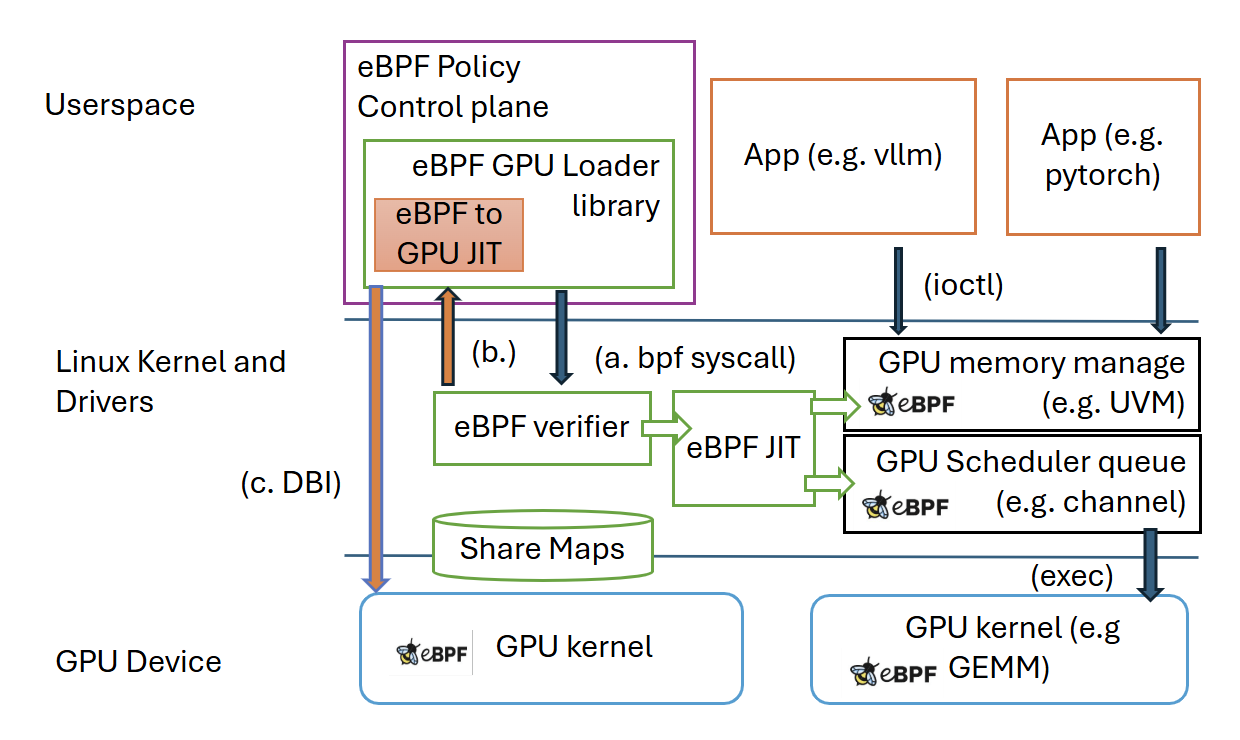
\includegraphics[width=\columnwidth]{img/gpu-ebpf-arch.png}
\vspace{-.5ex}
\caption{\sys high-level design: unified eBPF runtime spanning CPU and GPU.}
\label{fig:system-design}
\end{figure}

Figure~\ref{fig:system-design} shows the high-level architecture of \sys, composed of a user-space control plane and a unified kernel- and device-side execution path. \sys policies form distributed applications consisting of host- and device-side eBPF programs, hierarchical cross-layer maps, and a user-space control plane for lifecycle management.

\sys exposes \emph{hierarchical cross-layer maps}: logical eBPF map abstractions whose backing storage is automatically partitioned and replicated across host DRAM, GPU global memory, and optionally per-SM scratch space, with consistency and placement managed transparently by the runtime. Policy developers access maps via standard eBPF helpers regardless of execution context, without manual DMA transfers, memory placement, or address translation.

\paragraph{User-space Control Plane.}
Policy authors use standard eBPF tooling (e.g., \texttt{clang/libbpf}, \texttt{bpftool}) to build policy bytecode. The control-plane links against a loader library that installs policies and configures hierarchical maps. It enables runtime policy redeployment and reconfiguration (e.g., eviction thresholds, sampling rates, priorities) without application or kernel restarts, and exports runtime metrics (e.g., region hotness, tenant latencies) to external systems.

\paragraph{Kernel and Device Runtime.}
\sys provides a unified runtime across kernel and GPU contexts, managing verification, compilation, and map placement. It employs a SIMT-aware verifier (\S\ref{sec:verification}) that extends standard eBPF checks to reason about warp-uniformity, SIMT control flow, and GPU synchronization constraints. Verified programs are JIT-compiled into native host code or GPU-compatible instructions (e.g., PTX). The runtime manages hierarchical cross-layer maps as described above, dynamically optimizing placement based on access patterns and capacity constraints.

Policy execution occurs at structured hook points defined in GPU drivers and kernels. On the host, \sysdriver exposes \texttt{struct\_ops}-style hooks (e.g., region admission/eviction, kernel scheduling). Host handlers return concise policy decisions enforced via trusted kfuncs. On the GPU device, \sys injects lightweight trampolines at kernel entry/exit, warp synchronization barriers, and critical memory operations, invoking device-side handlers at warp granularity. Device handlers update cross-layer maps with performance signals (e.g., region access patterns, warp occupancy) and make granular control decisions (e.g., prefetch hints, block-level scheduling). Handlers never directly manipulate hardware registers or page tables; instead, they issue policy decisions via trusted helpers and kfuncs that the runtime enforces. GPU device eBPF also has access to general helpers like get time stamps.

% Together, the control-plane, unified runtime, and structured hook execution form an adaptive closed loop: device-side logic actively manages GPU resources and instrumentation; host-side handlers enforce global policies using shared instrumentation state; and the control-plane dynamically monitors and updates policies in real-time.

\subsection{Policy Interfaces}
\label{sec:design-interfaces}

\sys introduces three eBPF program types to categorize policy logic:
two driver-level types for GPU policy hooks (\texttt{BPF\_PROG\_TYPE\_GPU\_MEM} for memory events and \texttt{BPF\_PROG\_TYPE\_GPU\_SCHED} for scheduling) and one device-level type (\texttt{BPF\_PROG\_TYPE\_GPU\_DEV}) for GPU-kernel instrumentation. These types coexist with existing kernel eBPF program types (e.g., cgroup, TC) without conflict and are distinguished only by their attach points and SIMT-specific verifier rules.

\subsubsection{Memory Interface}
\label{sec:design-mem}

\sys treats memory placement as a programmable region
cache: it exposes a small set of region-level events for \emph{admission},
\emph{access}, and \emph{removal}, together with a prefetch channel, and lets host
and device cooperate on a unified policy.

On the host driver, these events are realized as a small \texttt{struct\_ops}-style policy
table with typed contexts:




\begin{minted}[
    highlightlines=false,
    fontsize=\footnotesize,
    breaklines=true,        % 开启自动换行
    breaksymbolleft=,       % 【关键】去除换行处的箭头符号
    breakindent=1em,        % 换行后缩进 1em，视觉上区分
    baselinestretch=0.9
]{c}
// Host-side policy callbacks for GPU memory management
struct gdrv_mem_ops {
  // Region created or eligible for device placement
  int (*region_add)(gdrv_mem_add_ctx_t *ctx);
  // Memory subsystem observes region use;
  // decide cache hit/eviction policies
  int (*region_access)(gdrv_mem_access_ctx_t *ctx);
  // Region about to leave device-resident working set
  int (*region_remove)(gdrv_mem_remove_ctx_t *ctx);
  // Safe points (kernel launches, faults) for prefetch
  int (*prefetch)(gdrv_mem_prefetch_ctx_t *ctx);
};

// Host-side kfuncs: reorder regions in eviction list
bool gdrv_mem_list_insert_head(gdrv_mem_list_t *list,
                               gmem_region_t *r);
bool gdrv_mem_list_insert_tail(gdrv_mem_list_t *list,
                               gmem_region_t *r);

// Device-side memory callback interface
struct gdev_mem_ops {
    // Warp observed memory access;
    void (*access)(gdev_mem_access_ctx_t *ctx);
    // Kernel provides
    void (*fence)(gdev_mem_fence_ctx_t *ctx);
};

// Device-side helpers
// Request prefetch, triggers callback in kernel
 int gdev_mem_prefetch(gmem_region_t* r);
\end{minted}

% map(address)

% // hostside
% prefetch_callback() {
% // check logic
%     prefetch region(device,address)
% }

% //device side
% SEC(gdev_entry/xxx)
% ebpf_gpu(int expert_id) {
%     gdev_mem_use_hint（address a, b)
% }
% // Pin memory on CPU or GPU
%  int gdev_mem_pin_hint(gmem_region_t* r, int dev_id);
% int gdev_mem_use_hint(gmem_region_t* r, int dev_id);


\paragraph{Host-side region events and decisions.}
On the host, \sys models memory as a set of logical regions and exposes attach points for three
canonical cache events. Handlers encode decisions via an enum field in the context (e.g., \texttt{ctx->decision = GDRV\_ADMIT} or \texttt{GDRV\_BYPASS}) and return 0 on success or a negative error code. \sys maintains all device-resident regions in a kernel-owned doubly linked list. The memory subsystem always inserts newly admitted regions at the tail and evicts from the head when under pressure. Even if eBPF handlers never select a region for eviction, memory pressure will still trigger kernel-driven FIFO eviction of head regions. eBPF handlers may only reorder regions via \texttt{gdrv\_mem\_list\_*} helpers; handlers cannot remove regions, and the kernel retains sole authority to evict. Together, these events realize a
general region-cache interface: policies implemented as eBPF handlers maintain their
own state in hierarchical maps (for example, MRU lists, LFU counters, or tenant budgets),
and respond to add/access/remove and prefetch callbacks with compact decisions. The underlying memory subsystem enforces these decisions
and maintains correct mappings, but delegates replacement and prefetch policy to
\sys.

\paragraph{Device-side memory events.}

On the GPU, \sys exposes a single device-side memory event interface that kernels
use both to report observed accesses and to express future-use hints. Device-side
handlers receive a compact, warp-uniform context struct with fields such as address , warp and SM identifiers. e.g. At selected memory operation sites, \sys injects lightweight hooks that operate at
warp granularity and invoke the device-side \texttt{access} handler.
% Each handler is verified to be warp-uniform and executes via a single warp-leader lane; other lanes remain idle at the hook, avoiding divergence and per-lane serialization (\S\ref{sec:verification}). The handler updates hierarchical maps with per-region statistics such as access counts, approximate working-set membership, and simple locality signatures.

The device-side interface also supports \emph{HINT} events, which device side eBPF 
invoke explicitly via helpers such as \texttt{gdev\_mem\_prefetch\_hint} and \texttt{gdev\_mem\_pin\_hint} when they have domain knowledge about future region usage. For
example, a mixture-of-experts kernel can compute the identifiers of experts it
will access for the next batch and call \texttt{gdev\_mem\_prefetch\_hint} to mark
the corresponding regions as ``will-use soon'';
a KV-cache kernel can emit hints that mark segments as cold and suitable for
demotion. device side HINT events like prefetch are recorded in control queues and can further trigger host side prefetch callbacks to do actual decisions.

\subsubsection{Scheduling Interface}
\label{sec:design-sched}

\sys exposes scheduling interfaces on both host and device so that policies can control
\emph{hardware queue lifecycle and properties} (context granularity) and \emph{how work is consumed inside kernels} (thread-block granularity), enabling priority-based scheduling and admission control while respecting the GPU execution model.

On the host, these lifecycle events are exported as a small struct-ops table of
scheduling callbacks:

\begin{minted}[highlightlines=false,fontsize=\footnotesize]{c}
// Host-side policy callbacks for GPU hardware
// queue scheduling
struct gdrv_sched_ops {
  // Hardware queue creation; set prio/timeslice,
  // return 0 to accept or <0 to reject/defer
  int  (*queue_create)(gsched_queue_ctx_t *ctx);
  // Hardware queue destruction; cleanup policy
  void (*queue_destroy)(gsched_queue_ctx_t *ctx);
};

// Host-side kfunc
bool gdrv_sched_preempt(gdrv_preempt_ctx_t *ctx);

// Device-side block scheduling callbacks
struct gdev_sched_ops {
  // Worker block starts/exits new work unit
  void (*enter)(gdev_block_ctx_t *ctx);
  void (*exit)(gdev_block_ctx_t *ctx);
  
  // Device function starts/ends
  void (*probe)(gdev_block_ctx_t *ctx);
  void (*retprobe)(gdev_block_ctx_t *ctx);
  
  // Return whether to steal work (TB scheduler)
  bool (*should_try_steal)(gdev_block_ctx_t *ctx);
};
\end{minted}

\paragraph{Host-side scheduling hooks.}
Modern GPU runtimes bypass the kernel for individual kernel launches, writing directly to command queues without syscalls. On the host, \sys exposes attach points for hardware queue lifecycle management. A hardware queue is the fundamental unit of GPU command submission, representing an independent channel bound to a process or context. The \texttt{queue\_create} handler is invoked when a new hardware queue is created; policies can set queue properties (e.g., priority, timeslice) via context fields and return 0 to accept or $<$0 to reject/defer creation, enabling admission control. The \texttt{queue\_destroy} handler runs when a queue is torn down, allowing policies to clean up associated state. Policies can also request preemption of an active queue via the \texttt{gdrv\_sched\_preempt} kfunc, which triggers a best-effort cooperative context switch. The host-side interface thus controls which queues exist, their scheduling properties, and how they are multiplexed across tenants. Thus, unlike user-space priority hints that driver may ignore, queue-level properties (priority, timeslice) are written directly into hardware scheduling structures and enforced by the GPU firmware, enabling policies to command rather than merely request scheduling behavior.

\paragraph{Device-side thread-block scheduler and signals.} Inside the GPU, \sys exposes a work stealing style interface that operates at the level of thread blocks or tiles, aligning with the SIMT execution model. Each kernel that uses \sys's internal scheduler is modeled as a pool of \emph{work units} (e.g., tiles or logical block indices) consumed by \emph{worker blocks}. Device-side policies observe and steer this internal scheduler via a \texttt{gdev\_block\_ctx} that includes the kernel identifier, tenant identifier, and a logical work-unit or block identifier. The verifier ensures that block-level scheduling decisions do not violate per-kernel invariants (e.g., blocks only select from their kernel's own work queue); detailed rules are described in \S\ref{sec:verification}. \sys support dynamic binary rewrite the kernel to use the thread block scheduler without source code access and recompile, or developer can integrate the scheduler framework themselves.


\subsection{Runtime Verification and Optimizations}
\label{sec:verification}

\sys policies execute directly within privileged GPU driver and kernel contexts, making strong safety guarantees essential. We adopt a standard eBPF threat model: we trust cluster operators loading policies, but consider policy code potentially buggy or misconfigured. The trusted computing base (TCB) includes the kernel eBPF verifier, \sys-specific kernel module, GPU runtime backend, and GPU driver/firmware. Policy authors only interact with eBPF abstractions and do not write native device code. For host-side verification, we reuse the existing Linux kernel eBPF verifier unchanged, relying on standard type-checking, bounded-loop, and memory-safety constraints. \sys-specific kfuncs and hooks are declared via BPF Type Format (BTF) metadata.

\subsubsection{SIMT-aware Verification}

A fundamental mismatch exists between traditional scalar eBPF semantics and GPU's SIMT parallel execution model. Directly executing scalar eBPF handlers on GPUs would severely degrade performance due to increased warp divergence and unbounded resource consumption. To address this, \sys introduces a novel SIMT-aware static verification model that rigorously enforces warp-level uniformity constraints and guarantees bounded resource usage.

The core insight is explicitly distinguishing \emph{warp-uniform} values (constant across all threads within a warp) from \emph{lane-varying} values (different per thread). Warp-uniform values are fields of the hook context that derive from driver or kernel state, such as region identifiers, kernel identifiers, tenant identifiers, or static configuration parameters. Lane-varying values arise from per-thread execution state, such as effective memory addresses, per-thread indices, or lane identifiers. We define a new type discipline integrated into the standard kernel eBPF verifier. The verifier performs a conservative dataflow analysis over the policy program to track the uniformity of each value. Context fields are annotated as uniform or varying via BTF metadata. Arithmetic and logical operations propagate these annotations: combining two uniform values yields a uniform result; any operation involving a varying operand yields a varying result; and helper or kfunc calls have their return uniformity declared in their specifications. The verifier enforces that critical control-flow decisions (branch conditions, loop bounds) strictly depend on warp-uniform variables. This constraint ensures that warp threads follow identical control paths, enabling safe and efficient warp-level aggregated execution. Lane-varying values are still permitted as inputs to arithmetic, aggregation, or summary computations; they simply cannot directly steer control flow.

The verifier further constrains side effects on shared state. Writes to shared eBPF maps and emission of hints or scheduling decisions must be expressible as warp-level operations: updates must be keyed by warp-uniform keys, and their values must be computed from warp-uniform quantities or warp-level aggregates of per-lane contributions. Direct per-lane updates to maps keyed by lane-varying values are rejected by the verifier.

Our verification model statically ensures safety-critical properties: bounded execution, no infinite loops or stalls, no unauthorized memory accesses, and freedom from prohibited synchronization operations. Each policy type has a per-program budget not only on eBPF instructions, but also on map operations, memory access helper calls, and memory operations per instruction to prevent policies from monopolizing GPU memory bandwidth. \sys also bans GPU-wide barriers and device-level synchronization constructs that could violate forward progress, as well as non-uniform atomic patterns that could introduce inter-warp dependency cycles. This explicit, GPU-specific extension of the eBPF verification model allows safe injection of programmable policies directly into privileged GPU driver and kernel contexts.

\subsubsection{Warp-level Execution Optimizations}

While SIMT-aware verification ensures correctness and safety, direct scalar execution of eBPF handlers across GPU threads would still incur prohibitive divergence and memory overhead. To eliminate this inefficiency, \sys introduces a novel warp-level aggregated execution model optimized specifically for GPU hardware characteristics.

The key idea is executing scalar policy logic exactly once per warp, using a designated ``warp leader'' thread. Conceptually, \sys divides each device-side hook invocation into a \emph{lane-local phase} and a \emph{warp-policy phase}. In the lane-local phase, each lane may perform scalar computation over its lane-varying inputs (effective addresses, per-thread indices) to produce per-lane contributions such as access counters or partial metrics. These computations must not influence control flow or directly update shared state. The results are then aggregated at warp scope using warp-level primitives (e.g., shuffle, ballot) to form warp-level summaries. In the warp-policy phase, the warp leader (typically lane~0) executes the GPU-side eBPF handler exactly once, using the warp-uniform context together with the aggregated summaries. The handler computes a warp-level decision and issues shared-state updates via approved helpers. Any per-lane effects are derived from this warp-level decision and broadcast back to all lanes. Under warp-uniform constraints enforced by the verifier, this aggregated warp-level execution preserves the original scalar eBPF semantics while drastically minimizing GPU overhead.

Additionally, recognizing that GPU policy code frequently accesses local, highly-thread-local map state, we perform aggressive specialization and inlining optimizations. These compiler-level optimizations eliminate unnecessary branching and helper call overhead, further reducing instruction count and warp divergence.

\subsubsection{Hierarchical Cross-layer Maps for State Coordination}

Effective GPU policy decisions require coherent sharing of policy state across asynchronous CPU and GPU execution contexts. As described in \S\ref{sec:arch}, \sys provides hierarchical cross-layer maps that transparently bridge CPU and GPU memory hierarchies. Logically, each map is a single key-value store accessible from host-side driver hooks, device-side handlers, and the user-space control plane. Physically, the runtime realizes a map as a hierarchy of shards distributed across host DRAM, GPU global memory, and on-chip memories such as shared memory or SM-local storage. The runtime dynamically manages map placement and synchronization based on access patterns, latency, and capacity constraints. For high-rate GPU-side updates (e.g., per-warp access counters), the runtime uses per-SM control queues that the host drains periodically, amortizing synchronization overhead while maintaining eventual consistency for host-side policy decisions.

\sys maps are designed explicitly as \emph{soft state}, following eBPF's philosophy of per-key atomicity and weak consistency. Each individual map lookup or update operation is atomic with respect to a given key, meaning policies never observe partially updated values. However, there are no global ordering guarantees across concurrent updates; if multiple contexts concurrently update the same key, the result is determined by the most recent writer. Rather than enforcing strong consistency, \sys provides a snapshot-based consistency model: device-side handlers perform frequent local updates, and the runtime periodically merges these into canonical map instances at well-defined merge points---typically at GPU kernel completion boundaries or explicitly triggered synchronization events. This relaxed model is adequate for policy decisions relying on aggregated statistics and approximate accounting. Stale data may degrade decision quality but cannot break correctness invariants like virtual address mappings or GPU memory integrity, which remain enforced by underlying driver and MMU mechanisms.
